\documentclass[a4paper,11pt,cours]{nsi} % COMPILE WITH DRAFT
\geometry{margin=2cm}
\usepackage{hyperref}
\usepackage{yhmath}
\usepackage{mathtools}

\begin{document}

\setcounter{chapter}{10} % 1 de moins que le num de chapitre

\chapter{Fonction exponentielle}

\section{Définition de la fonction exponentielle}
\begin{propriete}[]
	Il existe une unique fonction $f$ définie et dérivable sur $\R$ vérifiant : 
	$$\text{pour tout nombre réel }x  \quad f'(x)=f(x)\quad \text{et} \quad f(0)=1.$$
\end{propriete}
\begin{demonstration}
	L'existence de cette fonction est admise.\\
	La démonstration de l'unicité pourra être faite en exercice.
\end{demonstration}

\begin{definition}[ ]
	La \textbf{fonction exponentielle} est la fonction, notée $\exp$, définie et dérivable sur $\R$ telle que $\exp(0)=1 \ $ et $\ \exp'=\exp$.
\end{definition}

\begin{methode}[ ]
	\textbf{Déterminer la fonction $f$ définie et dérivable sur $\R$ telle que $f'=f$ et $f(0)=3$.}\\
	On pose : pour tout $x\in \R, f(x)=3\exp(x)$.\\
	Cette égalité définit la fonction $f$ qui est bien définie et dérivable sur $\R$.\\
	Pour $x\in \R, \quad f'(x)=3\exp'(x)=3\exp(x)=f(x)$.
\end{methode}


\section{Propriétés algébriques}
\begin{propriete}[ ]
	La fonction exponentielle est \textbf{strictement positive} : $\quad \text{pour tout } x\in \R,\ \exp(x)>0$.
\end{propriete}
%\newpage


\begin{demonstration}
	La démonstration pourra être faite en exercice.
\end{demonstration}

\begin{propriete}[ : Relation fonctionnelle]
	Pour tous nombres réels $x$ et $y$, $\quad \boxed{\exp(x+y)=\exp(x)\times \exp(y)}$.
\end{propriete}
\begin{demonstration}
	Soit $y$ un nombre réel fixé.\\
	On définit la fonction $f$ par : pour tout $x\in \R$, $\ f(x)=\dfrac{\exp(x+y)}{\exp(x)}$.\\
	$f$ est dérivable sur $\R$ comme quotient de fonctions dérivables sur $\R$ et, pour tout réel $x$, $$f'(x)=\dfrac{\exp(x+y)\exp(x)-\exp(x+y)\exp(x)}{\left[\exp(x)\right]^2}=0$$
	On en déduit que $f$ est une fonction \textbf{constante}. Ainsi, pour tout $x\in \R, \ f(x)=f(0)=\exp(y)$.\\
	On a donc montré que $\dfrac{\exp(x+y)}{\exp(x)}=\exp(y)$. Ainsi $\exp(x+y)=\exp(x)\times\exp(y)$.
\end{demonstration}

\begin{propriete}[ ]
	Pour tout nombre réel $x$, $\quad \exp(x)\times \exp(-x)=1 \quad$ et $\quad \exp(-x)=\dfrac{1}{\exp(x)}$.
\end{propriete}
\begin{demonstration}
	Soit $x$ un nombre réel.\\
	On applique le théorème précédent à $x$ et $-x$. On obtient :
	\begin{tabbing}
		$\exp(x)\times \exp(-x)$ \= $=\exp(x-x)$\\
		\>	$=\exp(0)$\\
		\>	$=1$
	\end{tabbing}
	Ainsi, pour tout $x\in \R$, $\exp(x)$ et $\exp(-x)$ sont inverses l'un de l'autre. Donc $\exp(-x)=\dfrac{1}{\exp(x)}$.
\end{demonstration}

\begin{propriete}[]
	Pour tous nombres réels $x$ et $y$, $\quad\exp(x-y)=\dfrac{\exp(x)}{\exp(y)}$.
\end{propriete}
%\newpage


\begin{demonstration}
	En exercice
\end{demonstration}

\begin{propriete}[ (admise)]
	Pour tout réel $x$ et tout entier relatif $n$, $\quad \boxed{\left[\exp(x)\right]^n=\exp(nx)}$.
\end{propriete}

\begin{exemple}[s]
\begin{multicols}{2}
	\begin{enumerate}[label=\textbullet]
		\item 	\begin{tabbing}
			$\exp(3)\times\exp(7)$	\= $=\exp(3+7)$\\
			\>	$=\exp(10)$
		\end{tabbing}
		\item 	$\exp(-5)=\dfrac{1}{\exp(5)}$
		\item	\begin{tabbing}
			$\left(\exp(2)\right)^4$	\= $=\exp(4\times 2)$\\
			\>	$=\exp(8)$
		\end{tabbing}
	\end{enumerate}	
\end{multicols}
\end{exemple}

\begin{exercice}[]
	Simplifier les expressions suivantes :
	\begin{multicols}{2}
		\begin{enumerate}[]
			\item 	$\exp(5)\times \exp(8) \times \left[\exp(2)\right]^3$\\[0.5em]
			\carreauxseyes{7.2}{3.2}
			\item 	$\exp(5)\times \left(\exp(5)\right)^{-1}\times\exp(10)$\\[0.5em]
			\carreauxseyes{7.2}{3.2}
		\end{enumerate}
	\end{multicols}
\end{exercice}

\section{Le nombre $e$}
\begin{definition}[ ]
	On note $\quad \exp(1)=e$
\end{definition}

\begin{remarque}[s]
	\begin{enumerate}[label=\textbullet]
		\item 	$e$ est un nombre réel irrationnel.
		\item 	$e \approx 2,718$
		\item	Pour tout $n\in\N, \quad \exp(n)=\exp(n\times 1)=\left[\exp(1)\right]^n=e^n$.	
	\end{enumerate}
\end{remarque}
	
\begin{notation}[ ]
	Par extension, pour tout $x\in \R$, on notera : $\quad \exp(x)=e^x$.
\end{notation}

\begin{propriete}[]
	Avec cette notation, les propriétés vues précédemment s'écrivent :\\
	Pour tous $x, y$ réels et tout $n$ entier relatif,
	\begin{multicols}{5}
		\begin{enumerate}[label=\textbullet]
			\item 	$e^{x+y}=e^x\times e^y$
			\item 	$e^x\times e^{-x}=1$
			\item	$e^{-x}=\dfrac{1}{e^x}$
			\item	$e^{x-y}=\dfrac{e^x}{e^y}$
			\item	$\left(e^x\right)^n=e^{nx}$
		\end{enumerate}
	\end{multicols} 
\end{propriete}

\begin{exemple}[]
	\begin{tabbing}
		$\dfrac{\left(e^7\right)^4\times e^3}{e^4}$	\= $=\dfrac{e^{7\times 4}\times e^3}{e^4}$\\[0.5em]
		\>	$=\dfrac{e^{28}\times e^3}{e^4}$\\[0.5em]
		\>	$=e^{28+3-4}$\\[0.5em]
		\>	$=e^{27}$
	\end{tabbing}
\end{exemple}

\section{La fonction exponentielle}

\begin{propriete}[]
	La fonction exponentielle est strictement croissante sur $\R$.
	\begin{center}
		\def\xmin{-5} \def\ymin{-1}\def\xmax{3}\def\ymax{5}
		\def\F{exp(\x)}
		\begin{tikzpicture}
			\clip (\xmin,\ymin) rectangle (\xmax,\ymax);
			\draw[fill = white] (\xmin,\ymin) rectangle (\xmax,\ymax);
			\repereal{\xmin}{\ymin}{\xmax}{\ymax}
			\draw[color=UGLiOrange,thick,domain=\xmin:3,smooth,variable=\x] plot ({\x},{\F});
			\draw[color=UGLiOrange] (2,4.5) node{\courbe{\exp}};
			\draw[color=olive] (4,4) node{(T)};
			\draw[color=olive,thick,domain=\xmin:\xmax,smooth,variable=\x] plot ({\x},{\x+1});
			\pointc{1}{2.718}{}{$e$}{$A$}
			
		\end{tikzpicture}
	\end{center}
\end{propriete}
%\newpage


\begin{demonstration}
	Pour tout $x\in\R, \exp'(x)=\exp(x)>0$.\\
	la fonction dérivée de la la fonction exponentielle est strictement positive sur $\R$ donc la fonction exponentielle est strictement croissante sur $\R$.
\end{demonstration}

\begin{propriete}[ ]
	Soient $a$ et $b$ deux nombres réels. On définit la fonction $f$ sur $\R$ par $\quad f(x)=e^{ax+b}$.\\
	La fonction $f$ est dérivable sur $\R$ et pour tout $x\in \R, \quad f'(x)=a\ e^{ax+b}$.
\end{propriete}
\begin{demonstration}
	Soient $a$ et $b$ deux nombres réels.\\
	On a vu dans le chapitre 8 que la dérivée de $f$ définie par $f(x)=g(ax+b)$ était donnée par : $\quad f'(x)=a\ g'(ax+b)$.\\
	On applique cette propriété avec $g=\exp$ et on obtient le résultat.
\end{demonstration}

\begin{exemple}[ ]
	\textbf{\'Etude des variations d'une fonction :}\\
	La fonction $h$ définie sur $\R$ par $\quad h(x)=-3\ e^{2x-5}+1\quad$ est dérivable sur $\R$ et pour tout $x\in\R$,
	\begin{tabbing}
		$h'(x)$	\= $=2\times \left(-3\ e^{2x-5}\right)+0$\\
		\>	$=-6\ e^{2x-5}$
	\end{tabbing}
	Pour tout $x\in\R, \quad e^{2x-5}>0,\quad$ donc $h'(x)<0$.\\
	La fonction $h$ est donc strictement décroissante sur $\R$.
\end{exemple}

\section{Applications : résolutions d'équations et d'inéquations}

\begin{propriete}[s]
Pour tous nombres réels $a$ et $b$ :
\begin{multicols}{2}
	\begin{enumerate}[label=\textbullet]
		\item 	$e^{a}=e^{b}\ \Leftrightarrow\ a=b$
		\item 	$e^{a}<e^{b}\ \Leftrightarrow\ a<b$
	\end{enumerate}
\end{multicols}
\end{propriete}

\begin{exemple}[s]
	\begin{multicols}{2}
		\begin{enumerate}[label=\textbullet]
			\item 	\textbf{Résolution d'équation :}\\
			Résoudre dans $\R \quad e^{2x}=\dfrac{1}{e}$ \\
			Soit $x\in\R$
			\begin{tabbing}
				$e^{2x}=\dfrac{1}{e} \quad$		\=	$\Leftrightarrow\quad e^{2x}=e^{-1}$\\
				
				\>	$\Leftrightarrow\quad 2x=-1$\\
				\>	$\Leftrightarrow \quad x=-\dfrac{1}{2}$
			\end{tabbing}
			L'équation $e^{2x}=\dfrac{1}{e}$ a pour unique solution $-\dfrac{1}{2}$.
			\vspace{0.8cm}
			\item	\textbf{Résolution d'inéquation :}\\
			Résoudre dans $\R \quad e^{-3x+4}+1\geqslant2$.\\
			Soit $x\in\R$.
			\begin{tabbing}
				$e^{-3x+4}+1\geqslant2 \quad$		\=	$\Leftrightarrow\quad e^{-3x+4}\geqslant1$\\
				
				\>	$\Leftrightarrow\quad  e^{-3x+4}\geqslant e^{0}$\\
				
				\> $\Leftrightarrow\quad -3x+4\geqslant 0$\\
				
				\> $\Leftrightarrow\quad x\leqslant\dfrac{4}{3}$
			\end{tabbing}
			L'ensemble des solutions de l'inéquation $e^{-3x+4}+1\geqslant2$ est l'intervalle $\oif{-\infty}{\dfrac{4}{3}}$.
		\end{enumerate}
	\end{multicols}
	
	
\end{exemple}
\newpage
\begin{aretenir}
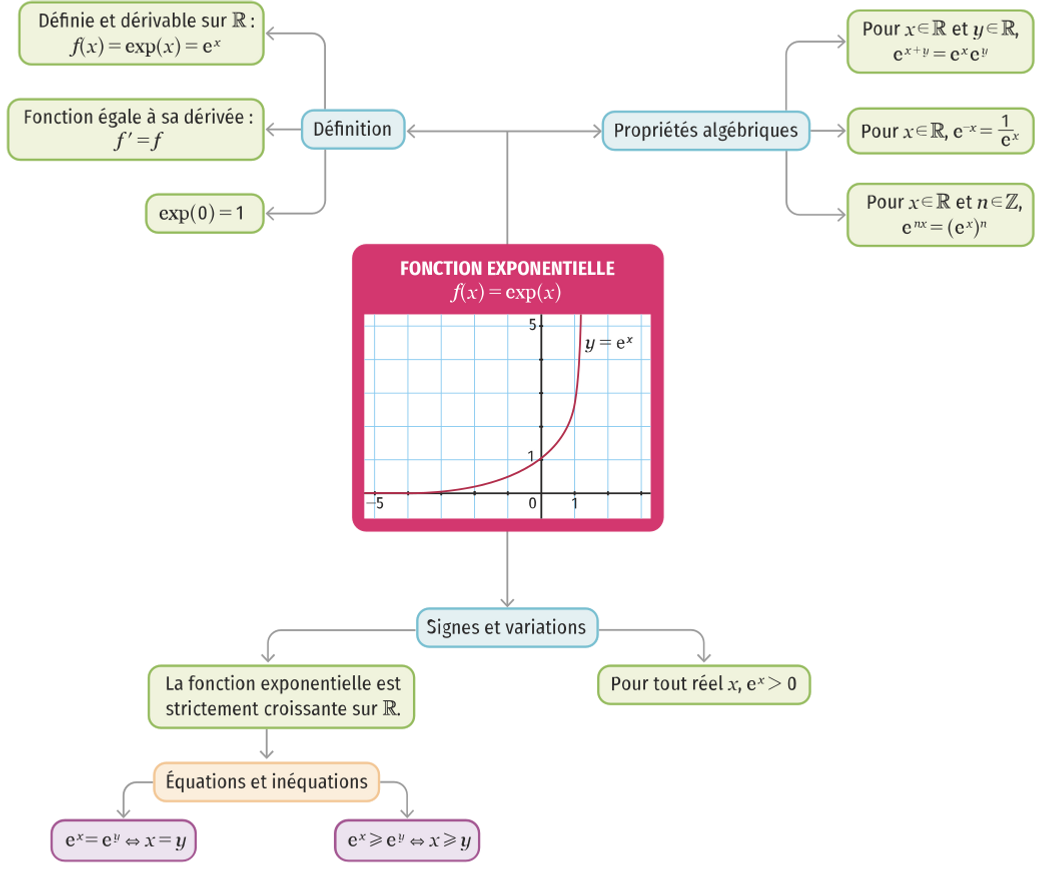
\includegraphics[width=16.5cm]{cartementale}
\end{aretenir}

\end{document}
